\section{Actividad 1}

\subsection*{Una antena transmisora emite una señal cosenoidal \( x(t) = A \cos(2\pi f_t t) \), donde \( A = 17 \, \text{W} \) y \( f_t = 532 \, \text{kHz} \). 
La antena receptora capta dos señales provenientes de dicha antena transmisora. La primera de ellas recorre el camino directo, con una distancia recorrida 
\( D_1 \). Mientras que la segunda, debido a una reflexión en un obstáculo, recorre una distancia \( D_2 \). Ambas señales sufren distintas atenuaciones, se 
suponen que son también aproximadamente cosenoidales y que viajan a la velocidad de la luz en el vacío, no sufriendo ninguna distorsión en su recorrido. Para 
el ejercicio debe considerarse los siguientes valores de atenuación y distancia:}

\begin{align*}
    A_1 &= 10\% & A_2 &= 25\% \\
    D_1 &= 11 \, \text{km} & D_2 &= 14.5 \, \text{km}
\end{align*}

\subsection*{a) Si las señales recibidas se suman en la antena receptora. ¿Cuál es el resultado de esto? Graficar. }

Las señales recibidas se expresan de la siguiente manera:

    \[
        y_1(t) = 0.9 \cdot 17 \cos(2\pi f_1 (t - \tau_1))
        \]
        \[
        y_2(t) = 0.75 \cdot 17 \cos(2\pi f_1 (t - \tau_2))
    \]

donde los retardos temporales son calculados como:

    \[
        \tau_1 = \frac{D_1}{c} = \frac{11000}{3 \times 10^8} = 36.67 \, \mu s
        \]
        \[
        \tau_2 = \frac{D_2}{c} = \frac{14500}{3 \times 10^8} = 48.33 \, \mu s
    \]

La señal resultante es la suma de la señal transmitida por un camino directo y de la señal reflejada \(y(t) = y_1(t) + y_2(t)\) 
\bigskip


\begin{figure}[H]
    \centering
        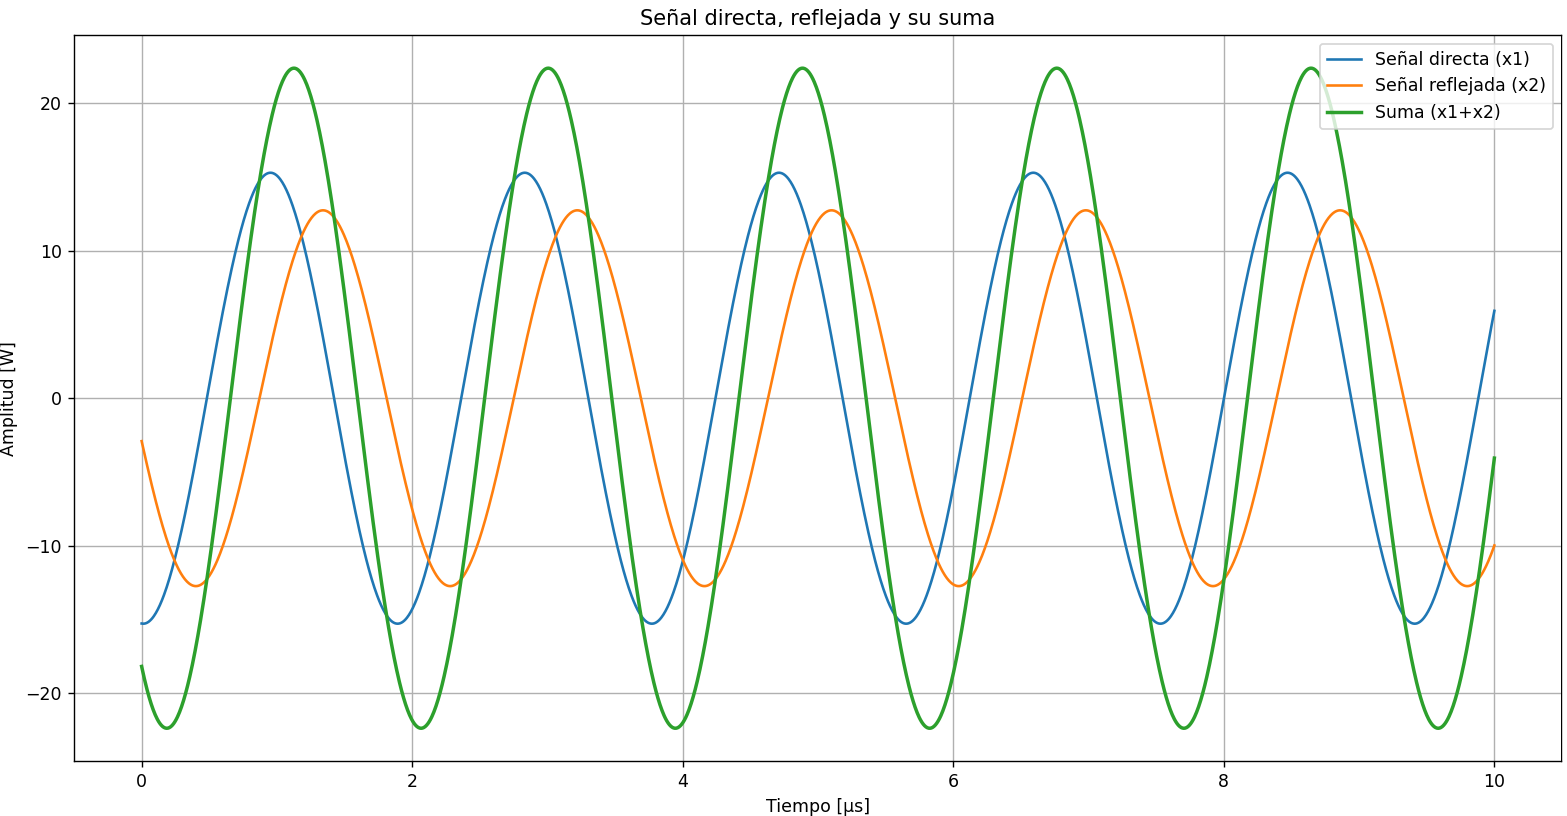
\includegraphics[width=0.8\textwidth]{imagenes/Actividad_1/grafico_532kHz.png}
        \caption{Señal resultante a 532 kHz.}
        \label{fig:532kHz}
    \end{figure}
\bigskip

En la Fig. \ref{fig:532kHz} se observa la señal cosenoidal trasmitida en su camino directo y reflejado, la suma de las dos es la que 
llega a la antena receptora. Como se observa, tienen diferente amplitud y fase debido a las atenuaciones y un retardo temporal por las 
diferentes distancias.
\bigskip

\subsection*{b) Suponer ahora que la frecuencia aumenta a 600 kHz. ¿Qué sucede? Graficar. }

Hay dos trayectorias:
    \[
         D_1 = \SI{11}{km} \qquad D_2 = \SI{14.5}{km}.  
    \]
\bigskip

La diferencia es:
    \[
        \Delta D = D_2 - D_1 = \SI{3.5}{km} = \SI{3500}{m}.
    \]
\bigskip

El retardo entre ambas:
    \[
        \Delta \tau = \frac{\Delta D}{c} = 
        \frac{3500}{3 \cdot 10^{8}}
        \approx 1.1667 \times 10^{-5}\,\text{s}.
    \]

\bigskip

La diferencia de fase entre ellas es:
    \[
        \Delta\varphi = 2\pi f \,\Delta\tau.
    \]


Las dos señales quedan en fase cuando su diferencia de fase es un múltiplo entero de \(2\pi\):
    \[
        \Delta\varphi = 2\pi n,\qquad n=0,1,2,\dots
    \]


    \[
        2\pi f \,\Delta\tau = 2\pi n \quad\Longrightarrow\quad f=\frac{n}{\Delta\tau}.
    \]
\bigskip

Para \(\Delta\tau=1.1667\times10^{-5}\,\text{s}\):
    \[
        f_n=\frac{n}{1.1667\times10^{-5}}.
    \]
\bigskip

Para \(n=7\):
    \[
        f_7=\frac{7}{1.1667\times10^{-5}}=600\,\text{kHz}.
    \]
\bigskip

A \(f=600\,\text{kHz}\) la diferencia de fase es:
    \[
        \Delta\varphi=2\pi f \,\Delta\tau=2\pi\cdot 600000\cdot1.1667\times10^{-5}
        =2\pi\cdot 7=14\pi,
    \]
que es exactamente 7 ciclos completos de diferencia. Por lo tanto, las señales quedan en fase. Por lo tanto, la señal resultante se 
observa en la Fig. \ref{fig:600kHz}.

    \begin{figure}[H]
        \centering
        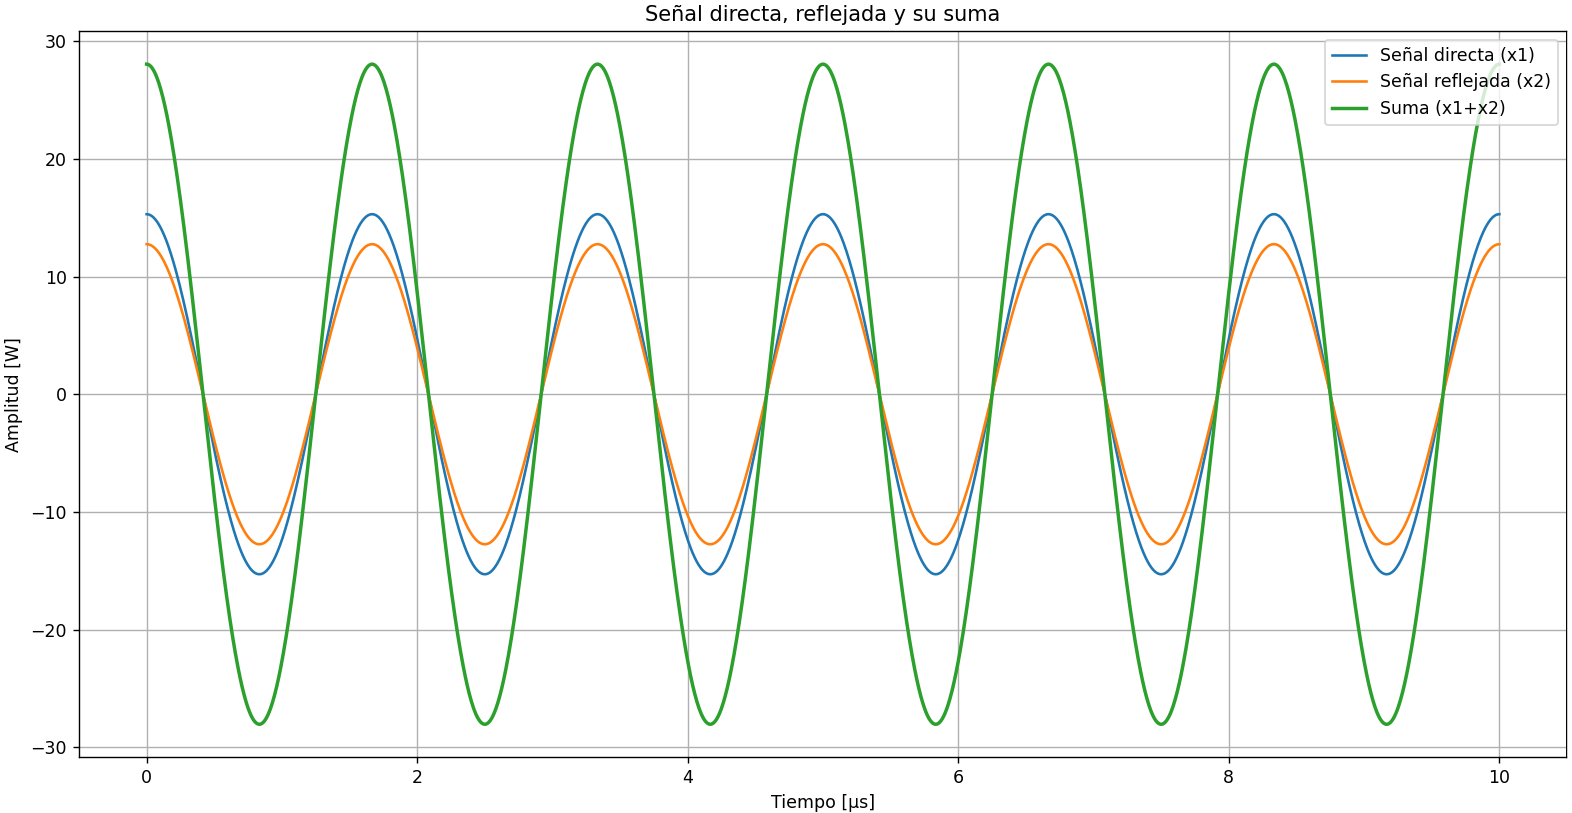
\includegraphics[width=0.8\textwidth]{imagenes/Actividad_1/grafico_600kHz.png}
        \caption{Señal resultante a 600 kHz.}
        \label{fig:600kHz}
    \end{figure}


\subsection*{c) Suponer que las señales sufren la misma atenuación. ¿Existe alguna frecuencia a la cual la señal recibida sea nula? Explicar el concepto.}

Cuando ambas señales sufren la misma atenuación, sus amplitudes se igualan, creando las condiciones ideales para que ocurra \textbf{interferencia destructiva 
total}. Para que la señal recibida sea nula, deben cumplirse dos condiciones fundamentales:

    \begin{enumerate}
        \item \textbf{Iguadad de amplitudes}: $A_1 = A_2$
        \item \textbf{Desfase de 180°}: $\Delta\phi = (2k+1)\pi$ rad, donde $k = 0, 1, 2, \ldots$
    \end{enumerate}

La diferencia de fase entre ambas señales está determinada por la relación:

    \[
        \Delta\phi = 2\pi f \frac{\Delta D}{c}
    \]

Donde:
    \begin{itemize}
        \item $\Delta D = D_2 - D_1 = 3.5 \, \text{km} = 3500 \, \text{m}$
        \item $c = 3 \times 10^8 \, \text{m/s}$
    \end{itemize}

Para obtener cancelación total:

    \[
        2\pi f \frac{\Delta D}{c} = (2k+1)\pi
    \]

Simplificando:

    \[
        2f \frac{\Delta D}{c} = 2k+1
    \]

    \[
        f = \frac{(2k+1)c}{2\Delta D}
    \]
Calculando las primeras tres frecuencias críticas donde se produce cancelación total:
    \begin{itemize}
        \item $k = 0$: $f_0 = \dfrac{3 \times 10^8}{7000} \approx 42.857 \, \text{kHz}$
        \item $k = 1$: $f_1 = \dfrac{3 \cdot 3 \times 10^8}{7000} \approx 128.571 \, \text{kHz}$
        \item $k = 2$: $f_2 = \dfrac{5 \cdot 3 \times 10^8}{7000} \approx 214.286 \, \text{kHz}$
    \end{itemize}

El fenómeno descrito constituye un caso clásico de \textbf{interferencia por multitrayectoria} en sistemas de comunicaciones. Las frecuencias en las que se 
produce cancelación total aparecen equiespaciadas en el dominio frecuencial, formando un patrón periódico cuya periodicidad depende directamente de la 
diferencia de caminos $\Delta D$. Matemáticamente, existe un conjunto infinito y discreto de frecuencias críticas dadas por la expresión:

\[
f_k = \frac{(2k+1)c}{2\Delta D}, \quad k = 0, 1, 2, \ldots
\]

donde $c$ es la velocidad de la luz. Este resultado tiene implicancias directas en el diseño de sistemas de comunicación, donde resulta esencial evitar la 
transmisión en dichas frecuencias críticas o, alternativamente, implementar técnicas de diversidad como el uso de múltiples antenas o saltos en frecuencia 
para mitigar los efectos adversos de la interferencia por multitrayectoria.
